%% -*- fill-column: 79; -*-

\def\currentprefix{enemy}


%% listing settings
\lstset{ %
language=Ruby,                % the language of the code
basicstyle=\footnotesize\ttfamily,       % the size of the fonts that are used for the code
escapeinside={\%*}{*)},         % if you want to add a comment within your code
morekeywords={*,...},           % if you want to add more keywords to
}


%% \widowpenalty=10000
%% \clubpenalty=10000




%% \begin{document}

%% \date{}

%% \title{Enemy of the State:\\
%%    A State-Aware Black-Box Web Vulnerability Scanner  
%% }

%% \author{
%%   {\rm Adam Doup\'e, Ludovico Cavedon, Christopher Kruegel, and Giovanni Vigna}\\
%%   University of California, Santa Barbara\\
%%   {\rm \texttt{\{adoupe, cavedon, chris, vigna\}@cs.ucsb.edu}}
%% }

%% \maketitle

% Use the following at camera-ready time to suppress page numbers.
% Comment it out when you first submit the paper for review.
%\thispagestyle{empty}


%% \subsection*{Abstract}

%% Black-box web vulnerability scanners are a popular choice for finding security
%% vulnerabilities in web applications in an automated fashion. These tools
%% operate in a \emph{point-and-shoot} manner, testing any web
%% application---regardless of the server-side language---for common security
%% vulnerabilities. Unfortunately, black-box tools suffer from a number of
%% limitations, particularly when interacting with complex applications that have
%% multiple actions that can change the application's state. If a vulnerability
%% analysis tool does not take into account changes in the web application's
%% state, it might overlook vulnerabilities or completely miss entire portions of
%% the web application.

%% We propose a novel way of inferring the web application's internal state
%% machine \emph{from the outside}---that is, by navigating through the web
%% application, observing differences in output, and incrementally producing a
%% model representing the web application's state.

%% We utilize the inferred state machine to drive a black-box web application
%% vulnerability scanner. Our scanner traverses a web application's state machine
%% to find and fuzz user-input vectors and discover security flaws. We implemented our technique in a prototype
%% crawler and linked it to the fuzzing component from an open-source web
%% vulnerability scanner.

%% We show that our state-aware black-box web vulnerability scanner is able to not
%% only exercise more code of the web application, but also discover
%% vulnerabilities that other vulnerability scanners miss.

Web applications are the most popular way of delivering services via the
Internet. A modern web application is composed of a back-end, server-side part
(often written in Java or in interpreted languages such as PHP, Ruby, or
Python) running on the provider's server, and a client part running in the
user's web browser (implemented in JavaScript and using HTML/CSS for
presentation). The two parts often communicate via HTTP over the Internet using
Asynchronous JavaScript and XML (AJAX)~\cite{garrett05:ajax}.

The complexity of modern web applications, along with the many different
technologies used in various abstraction layers, are the root cause of
vulnerabilities in web applications. In fact, the number of reported web
application vulnerabilities is growing sharply~\cite{steve07,
  fossi09:symantec}.

The occurrence of vulnerabilities could be reduced by better education of web
developers, or by the use of security-aware web application development
frameworks~\cite{robertson09, chong07}, which enforce separation between
structure and content of input and output data. In both cases, more effort and
investment in training is required, and, therefore, cost and time-to-market
constraints will keep pushing for the current fast-but-insecure development
model.

A complementary approach for fighting security vulnerabilities is to discover and
patch bugs before malicious attackers find and exploit them. One way is to use
a white-box approach, employing static analysis of the source
code~\cite{felmetsger10:logic,huang03:web,jovanovic10:static,balzarotti08:saner}.
There are several drawbacks to a white-box approach. First, the potential
applications that can be analyzed is reduced to only those applications that
use the target programming language. In addition, there is the problem of
substantial false positives. Finally, the source code of the
application itself may be unavailable.

The other approach to discovering security vulnerabilities in web applications
is by observing the application's output in response to a specific input. This
method of analysis is called \emph{black-box} testing, as the application is
seen as a sealed machine with unobservable internals. Black-box approaches are
able to perform large-scale analysis across a wide range of applications. While
black-box approaches usually have fewer false positives than white-box
approaches, black-box approaches suffer from a discoverability problem: They
need to reach a page to find vulnerabilities on that page.

Classical black-box web vulnerability scanners crawl a web application to
enumerate all reachable pages and then fuzz the input data (URL parameters,
form values, cookies) to trigger vulnerabilities. However, this approach
ignores a key aspect of modern web applications: Any request can change the state of the web application.

In the most general case, the state of the web application is any data
(database, filesystem, time) that the web application uses to determine
its output. Consider a forum that authenticates users, an e-commerce
application where users add items to a cart, or a blog where visitors and
administrators can leave comments. In all of these modern applications, the way
a user interacts with the application determines the application's state.

Because a black-box web vulnerability scanner will never detect a vulnerability
on a page that it does not see, scanners that ignore a web application's state
will only explore and test a (likely small) fraction of the web application.

In this chapter, we propose to improve the effectiveness of black-box web vulnerability scanners by
increasing their capability to understand the web application's internal state.
Our tool constructs a partial model of the web application's state machine in a
fully-automated fashion. It then uses this model to fuzz the application in a
state-aware manner, traversing more of the web application and thus discovering
more vulnerabilities.

\noindent{}The main contributions of this chapter are the following:
\begin{itemize}
 \item A black-box technique to automatically learn a model of a web
   application's state. 
 \item A novel vulnerability analysis technique that leverages the web
   application's state model to drive fuzzing.
 \item An evaluation of our technique, showing that both code coverage and
   effectiveness of vulnerability analysis are improved.
\end{itemize}

\section{Motivation}
\begin{figure}[tb]
  \centering
  \resizebox{0.45\textwidth}{!}{
\begin{tikzpicture}[>=latex,line join=bevel,]
%%
\begin{scope}
  \pgfsetstrokecolor{black}
  \definecolor{strokecol}{rgb}{1.0,1.0,1.0};
  \pgfsetstrokecolor{strokecol}
  \definecolor{fillcol}{rgb}{1.0,1.0,1.0};
  \pgfsetfillcolor{fillcol}
  \filldraw (0bp,0bp) -- (0bp,61bp) -- (174bp,61bp) -- (174bp,0bp) -- cycle;
\end{scope}
  \node (index) at (139bp,10bp) [draw,ellipse] {index.php};
  \node (login) at (34bp,10bp) [draw,ellipse] {login.php};
  \node (view) at (139bp,50bp) [draw,ellipse] {view.php};
  \draw [->] (index) ..controls (98.315bp,16.8bp) and (84.39bp,16.941bp)  .. (login);
  \draw [->] (view) ..controls (113.62bp,36.131bp) and (111.25bp,31.205bp)  .. (index);
  \draw [->] (login) ..controls (73.167bp,3.2414bp) and (87.055bp,3.0553bp)  .. (index);
  \draw [->] (index) ..controls (164.47bp,23.988bp) and (166.76bp,28.914bp)  .. (view);
%
\end{tikzpicture}

}
  \caption{Navigation graph of a simple web application.}
  \locallabel{simple-nav-graph}
\end{figure}

\begin{figure}[tb]
  \centering
  \resizebox{0.8\textwidth}{!}{
\begin{tikzpicture}[>=latex,line join=bevel,]
%%
\node (S-_0) at (27.5bp,10.5bp) [draw,ellipse] {S\_0};
  \node (S-_1) at (141.5bp,10.5bp) [draw,ellipse] {S\_1};
  \draw [->] (S-_0) ..controls (61.199bp,10.5bp) and (93.88bp,10.5bp)  .. (S-_1);
  \definecolor{strokecol}{rgb}{0.0,0.0,0.0};
  \pgfsetstrokecolor{strokecol}
  \draw (84.5bp,21bp) node {login.php};
  \draw [->] (S-_0) ..controls (14.375bp,27.375bp) and (17bp,37.5bp)  .. (27.5bp,37.5bp) .. controls (34.062bp,37.5bp) and (37.549bp,33.545bp)  .. (S-_0);
  \draw (27.5bp,48bp) node {index.php};
  \draw [->] (S-_1) ..controls (128.38bp,27.375bp) and (131bp,37.5bp)  .. (141.5bp,37.5bp) .. controls (148.06bp,37.5bp) and (151.55bp,33.545bp)  .. (S-_1);
  \draw (141.5bp,48bp) node {index.php};
  \draw [->] (S-_1.east) ..controls (165.83bp,19.5bp) and (184.5bp,19.5bp)  .. (184.5bp,10.5bp) .. controls (184.5bp,3.8203bp) and (174.22bp,2.0982bp)  .. (S-_1.east);
  \draw (210.5bp,10.5bp) node {view.php};
%
\end{tikzpicture}

}
  \caption{State machine of a simple web application.}
  \locallabel{simple-state-graph}
\end{figure}


Crawling modern web applications means dealing with the web application's
changing state. Previous work in detecting workflow
violations~\cite{balzarotti07:mimosa,li11:BLOCK,cova07:swaddler,felmetsger10:logic}
focused on navigation, where a malicious user can access a page that is
intended only for administrators. This unauthorized access is a violation of
the developer's intended work-flow of the application.

We wish to distinguish a navigation-based view of the web application, which is
simply derived from crawling the web application, from the web application's
internal state machine. To illustrate this important difference, we will use a small
example.

Consider a simple web application with three pages,
\texttt{index.php}, \texttt{login.php}, and \texttt{view.php}. The
\texttt{view.php} page is only accessible after the \texttt{login.php} page is
accessed. There is no logout functionality. A client accessing this web
application might make a series of requests like the following:

\noindent{}$\langle$\texttt{index.php}, \texttt{login.php}, \texttt{index.php},
\texttt{view.php}, \\
\phantom{$\langle$}\texttt{index.php}, \texttt{view.php}$\rangle$

Analyzing this series of requests from a navigation perspective creates a
navigation graph, shown in Figure~\localref{simple-nav-graph}. This graph shows
which page is accessible from every other page, based on the navigation trace.
However, the navigation graph does not represent the information that
\texttt{view.php} is only accessible after accessing \texttt{login.php}, or
that \texttt{index.php} has changed after requesting \texttt{login.php} (it
includes the link to \texttt{view.php}).

What we are interested in is not how to navigate the web application, but how
the requests we make influence the web application's internal state machine.
The simple web application described previously has the internal state machine shown
in Figure~\localref{simple-state-graph}. The web application starts with the internal
state \texttt{S\_0}. Arrows from a state show how a request affects the web
application's internal state machine. In this example, in the initial state,
\texttt{index.php} does not change the state of the application, however,
\texttt{login.php} causes the state to transition from \texttt{S\_0} to
\texttt{S\_1}. In the new state \texttt{S\_1}, both \texttt{index.php} and
\texttt{view.php} do not change the state of the web application.

The state machine in Figure~\localref{simple-state-graph} contains important
information about the web application. First, it shows that \texttt{login.php}
permanently changes the web application's state, and there is no way to recover
from this change. Second, it shows that the \texttt{index.php} page is seen in
two different states.

Now the question becomes: ``How does knowledge of the web application's state
machine (or lack thereof) affect a black-box web vulnerability scanner?'' The
scanner's goal is to find vulnerabilities in the application, and to do so it
must fuzz as many execution paths of the server-side code as
possible\footnote{Hereinafter, we assume that the scanner relies on
  fuzzer-based techniques. However, any other automated vulnerability analysis
  technique would benefit from our state-aware approach.}. Consider the simple
application described in Figure~\localref{simple-state-graph}. In order to fuzz as
many code paths as possible, a black-box web vulnerability scanner must fuzz
the \texttt{index.php} page in both states \texttt{S\_0} and \texttt{S\_1},
since the code execution of \texttt{index.php} can follow different code paths
depending on the current state (more precisely, in state \texttt{S\_1},
\texttt{index.php} includes a link to \texttt{view.php}, which is not present
in \texttt{S\_0}).

A black-box web vulnerability scanner can also use the web application's state
machine to handle requests that change state. For example, when fuzzing the
\texttt{login.php} page of the sample application, a fuzzer will try to make
several requests to the page, fuzzing different parameters. However, if the
first request to \texttt{login.php} changes the state of the application, all
further requests to \texttt{login.php} will no longer execute along the same
code path as the first one. Thus, a scanner must have knowledge of the web
application's state machine to test if the state was changed, and if it was,
what requests to make to return the application to the previous state before
continuing the fuzzing process.

We have shown how a web application's state machine can be leveraged to improve
a black-box web vulnerability scanner. Our goal is to infer, in a black-box
manner, as much of the web application's state machine as possible. Using only
the sequence of requests, along with the responses to those requests, we build
a model of as much of the web application's state machine as possible. In the
following section, we describe, at a high level, how we infer the web
application's state machine. Then, in Section~\localref{details}, we provide the
details of our technique.

\section{State-Aware Crawling}

In this section, we describe our state-aware crawling approach. In
Section~\localref{webapps}, we describe web applications and define terms that we
will use in the rest of the chapter. Then, in Section~\localref{inferring}, we
describe the various facets of the state-aware crawling algorithm at a high
level.
%% - Start with model of web applications.
%% - Describe how we detect state changes via the model.
%% - Next, how we explore and find the next link.
%% - Page clusterer is important to detect state change
%% - Why is request clustering important?
%% - Form Filling is important for coverage
%% - When to quit important for completion.
%% High level overview
%% High level Steps
%% Sections for each part of the algorithm

\subsection{Web Applications}
\locallabel{webapps}

Before we can describe our approach to inferring a web application's state, we
must first define the elements that come into play in our web application model.

A web application consists of a server component, which accepts HTTP requests.
This server component can be written in any language, and could use many
different means of storage (database, filesystem, memcache). After
processing a request, the server sends back a response. This response
encapsulates some content, typically HTML. The HTML content contains links and
forms which describe how to make further requests. 

Now that we have described a web application at a high level, we need to define
specific terms related to web applications that we use in the rest of this chapter.

\begin{itemize}

\item Request---The HTTP request made to the web application. Includes anything
  (typically in the form of HTTP headers) that is sent by the user to the web
  application: the HTTP Method, URL, Parameters (\texttt{GET} and \texttt{POST}), Cookies, and
  User-Agent.

\item Response---The response sent by the server to the user. Includes
  the HTTP Response Code and the content (typically HTML).

\item Page---The HTML page that is contained in the response from a web
  application.

\item Link---Element of an HTML page that tells the browser how to create a
  subsequent request. This can be either an anchor or a form. An anchor always
  generates a \texttt{GET} request, but a form can generate either a
  \texttt{POST} or \texttt{GET} request, depending on the parameters of the
  form.

\item State---Anything that influences the web application's server-side code execution.

\end{itemize}

\subsubsection{Web Application Model}
\locallabel{webappmodel}

\begin{figure}[tb]
  \centering
  \resizebox{\textwidth}{!}{\begin{figure*}[tb]
  \centering
  \includegraphics{figures/complicated_state_machine.ps}
  \caption{The state machine of a simple e-commerce application.}
  \locallabel{complicated-state-machine}
\end{figure*}
}
  \caption{The state machine of a simple e-commerce application.}
  \locallabel{complicated-state-machine}
\end{figure}


We use a \emph{symbolic Mealy machine}~\cite{berg08} to model the web
application as a black-box. A Mealy machine is an automaton where the input to
the automaton, along with the current state, determines the output (i.e., the
page produced by the response) and the next state. A Mealy machine operates on a
finite alphabet of input and output symbols, while a symbolic Mealy machine uses
an infinite alphabet of input and output symbols.

This model of a web application works well because the input to a web
application, along with the current state of the web application, determines
the output and the next state. Consider a simple e-commerce web application
with the state machine show in Figure~\localref{complicated-state-machine}. In this
state graph, all requests except for the ones leaving a state bring the
application back to the same state. Therefore, this state graph does not show
all the request that can be made to the application, only the subset of
requests that change the state.

For instance, in the initial state \texttt{S\_0}, there is only one request that
will change the state of the application, namely \texttt{POST~/login.php}. This
change logs the user into the web application. From the state
\texttt{no\_items}, there are two requests that can change the state,
\texttt{GET~/logout.php} which returns the user to the initial state \texttt{S\_0} and
\texttt{POST~/add\_item.php} to add an item to the user's shopping cart.

Note that the graph shown in Figure~\localref{complicated-state-machine} is not a
strongly connected graph---that is, every state cannot be reached by every
other state. In this example, purchasing an item is a permanent action, it
irrecoverably changes the state (there is no link from
\texttt{purchased\_item} to \texttt{item\_in\_cart}). Another interesting
aspect is that one request, \texttt{GET~/logout.php}, leads to three different
states. This is because once the web application's state has changed, 
logging out, and then back in, does not change the state of the cart.

\subsection{Inferring the State Machine}
\locallabel{inferring}

Inferring a web application's state machine requires the ability to detect when
the state of the web application has changed. Therefore, we start with a
description of the state-change detection algorithm, then explain the other
components that are required to infer the state machine. 

The key insight of our state-change algorithm is the following: We detect
that the state of the web application has changed when we make an identical
request and get a different response. This is the only externally visible
effect of a state-change: Providing the same input causes a different output.

Using this insight, our state-change detection algorithm works, at a high level,
as follows: (1) Crawl the web application sequentially, making requests based on
a link in the previous response. (2) Assume that the state stays the same,
because there is no evidence to the contrary. (3) If we make a request identical
to a previous request and get a different response, then we assume that some
request since the last identical request changed the state of the web
application.

The intuition here is that a Mealy machine will, when given the same input in
the same state, produce the same output. Therefore, if we send the same request
and get a different output, the state must have changed. By detecting the web
application's state changes only using inputs and outputs, we are agnostic with
respect to both \emph{what} constitutes the state information and \emph{where}
the state information is located. In this way, we are more generic than
approaches that only consider the database to hold the state of the
application, when in fact, the local file system or even memory could hold part
of the web application's state.

The state-change detection algorithm allows us to infer when the web
application's state has changed, yet four other techniques
are necessary to infer a state machine: the clustering of
similar pages, the identification of state-changing requests, the collapsing of
similar states, and navigating.

\noindent \textbf{Clustering similar pages.}
We want to group together pages that are similar, for two reasons: To handle
infinite sections of web applications that are generated from the same
code (e.g., the pages of a calendar) and to detect when a response has changed.

Before we can cluster pages, we model them using the links (anchors and forms) present on
the page. The intuition here is that the links describe \emph{how}
the user can interact with the web application. Therefore, changes to what a
user can do (new or missing links) indicate when the state of the web
application has changed. Also, infinite sections of a web application will
share the same link structure and will cluster together. 

With our page model, we cluster pages together based on their link structure.
Pages that are in different clusters are considered different. The details of
this approach are described in Section~\localref{page-clustering}.

\noindent \textbf{Determining the state-changing request.}
The state-change detection algorithm only says that the state has changed, however we
need to determine \emph{which} request actually changed the state. When we
detect a state change, we have a temporal list of requests with
identical requests at the start and end. One of the requests in this list
changed the state. We use a heuristic to determine which request changed the
state. This heuristic favors newer requests over older requests, \texttt{POST}
requests over \texttt{GET} requests, and requests that have previously changed
the state over those that have never changed the state. The details are
described in Section~\localref{par:statechangedet}.

\noindent \textbf{Collapsing similar states.}
The state-change detection algorithm detects only when the state has changed, however, we
need to understand if we returned to a previous state. This is necessary
because if we detect a state change, we want to know if this is a state we
have previously seen or a brand new state. We reduce this problem to a graph coloring problem, where the
nodes are the states and an edge between two nodes means that the states cannot
be the same. We add edges to this graph by using the requests and responses,
along with rules to determine when two states cannot be the same. After the
graph is colored, states that are the same color are collapsed into the same
state. Details of this state-merging technique are provided in Section~\localref{collapsing-similar-states}.

\noindent \textbf{Navigating.}
We have two strategies for crawling the web application.

First, we always try to pick a link in the last response. The rational behind choosing a
link in the last response is that we emulate a user browsing the web application.
In this way, we are able to handle multi-step processes, such as previewing a
comment before it is committed.

Second, for each state, we make requests that are the least likely to change
the state of the web application. The intuition here is that we want to first see
as much of a state as possible, without accidentally changing the state, in
case the state change is permanent. Full details of how we crawl the web
application are provided in Section~\localref{navigation}

\section{Technical Details}
\locallabel{details}

Inferring a web application's state machine requires concretely defining
aspects such as page clustering or navigation. However, we wish to stress that
this is one implementation of the state machine inference algorithm and it may
not be optimal.

\subsection{Clustering Similar Pages}
\locallabel{page-clustering}

Our reason for grouping similar pages together is twofold: Prevent infinite
scanning of the website by grouping the ``infinite'' areas together and detect
when the state has changed by comparing page responses in an efficient manner.

\subsubsection{Page Model}\locallabel{par:pagemodel}
\begin{figure}[tb]
  \centering
  \resizebox{0.8\textwidth}{!}{
\begin{tikzpicture}[>=latex,line join=bevel,]
%%
\node (11) at (149bp,250bp) [draw,ellipse] {/html/body/div/span/a};
  \node (51) at (14bp,12bp) [draw,ellipse] {(0)};
  \node (12) at (319bp,250bp) [draw,ellipse] {/html/body/div/form};
  \node (21) at (149bp,190bp) [draw,ellipse] {/user};
  \node (22) at (319bp,190bp) [draw,ellipse] {/post};
  \node (55) at (319bp,12bp) [draw,ellipse] {(5)};
  \node (32) at (319bp,131bp) [draw,ellipse] {edit.php};
  \node (31) at (149bp,131bp) [draw,ellipse] {profile.php};
  \node (42) at (178bp,72bp) [draw,ellipse] {(all, sorted)};
  \node (43) at (319bp,72bp) [draw,ellipse] {(text, email, id)};
  \node (53) at (122bp,12bp) [draw,ellipse] {(5)};
  \node (41) at (73bp,72bp) [draw,ellipse] {(id, page)};
  \node (54) at (184bp,12bp) [draw,ellipse] {(NULL)};
  \node (52) at (68bp,12bp) [draw,ellipse] {(0, 1)};
  \node (Page) at (234bp,309bp) [draw,ellipse] {Page};
  \draw [->] (41) ..controls (53.165bp,51.501bp) and (40.2bp,38.756bp)  .. (51);
  \draw [->] (32) ..controls (319bp,112.78bp) and (319bp,103.19bp)  .. (43);
  \draw [->] (22) ..controls (319bp,170.44bp) and (319bp,160.72bp)  .. (32);
  \draw [->] (21) ..controls (149bp,170.44bp) and (149bp,160.72bp)  .. (31);
  \draw [->] (43) ..controls (319bp,52.596bp) and (319bp,42.968bp)  .. (55);
  \draw [->] (31) ..controls (157.86bp,112.59bp) and (163.2bp,102.09bp)  .. (42);
  \draw [->] (Page) ..controls (209.63bp,291.66bp) and (189.45bp,278.12bp)  .. (11);
  \draw [->] (31) ..controls (125.18bp,112.13bp) and (108.37bp,99.527bp)  .. (41);
  \draw [->] (11) ..controls (149bp,230.6bp) and (149bp,220.97bp)  .. (21);
  \draw [->] (12) ..controls (319bp,230.6bp) and (319bp,220.97bp)  .. (22);
  \draw [->] (Page) ..controls (258.37bp,291.66bp) and (278.55bp,278.12bp)  .. (12);
  \draw [->] (41) ..controls (89.167bp,51.863bp) and (99.367bp,39.79bp)  .. (53);
  \draw [->] (42) ..controls (179.9bp,52.596bp) and (180.9bp,42.968bp)  .. (54);
  \draw [->] (41) ..controls (71.413bp,52.596bp) and (70.583bp,42.968bp)  .. (52);
%
\end{tikzpicture}

}
  \caption{Representation of a page's link vectors stored in
    a prefix tree. There are five links present on this tree, as
    evidenced by the number of leaf nodes.}
  \locallabel{page-prefix-tree}
\end{figure}

\begin{figure*}[tb]
  \centering
  \resizebox{\textwidth}{!}{\begin{figure*}[tb]
  \centering
  \includegraphics{figures/abstract_page_tree.ps}
  \caption{Abstract Page Tree. Every page's link vector is stored
    in this prefix tree. There are seven pages in this tree. The page link vector
    from Figure~\localref{page-prefix-tree} is highlighted in bold.}
  \locallabel{abstract-page-tree}
\end{figure*}
}
  \caption{Abstract Page Tree. Every page's link vector is stored
    in this prefix tree. There are seven pages in this tree. The page link vector
    from Figure~\localref{page-prefix-tree} is highlighted in bold.}
  \locallabel{abstract-page-tree}
\end{figure*}


The output of a web application is usually an HTML document (it can actually be
any arbitrary content, but we only consider HTML content and HTTP redirects).
An HTML page is composed of navigational information (anchors and forms) and
user-readable content. For our state-change detection algorithm, we are not
interested in changes to the content, but rather to changes in the navigation
structure. We focus on navigation changes because the links on a page define
how a user can interact with the application, thus, when the links change, the
web application's state has changed.

Therefore, we model a page by composing all the anchors and forms. First, every
anchor and form is transformed into a vector constructed as follows:
\[
\langle{}dompath,\ action,\ params,\ values\rangle{}
\]
where:
\begin{itemize}
 \item $dompath$ is the DOM (\emph{Document Object Model}) path of the HTML
  link (anchor or form);
 \item $action$ is a list where each element is from the \texttt{href} (for anchors) or
  \texttt{action} (for forms) attribute split by `/';
 \item $params$ is the (potentially empty) set of parameter names of the form
   or anchor;
 \item $values$ is the set of values assigned to the parameters listed in
   $params$.
\end{itemize}

\noindent{}For instance, an anchor tag with the \texttt{href} attribute of
\path{/user/profile.php?id=0&page} might have the following link vector:%
\[\langle{}\text{/html/body/div/span/a},\ \text{/user},\ \text{profile.php},\ \text{(id,
  page)},\ \text{(0)}\rangle{}\] 

All link vectors of a page are then stored in a prefix tree. This prefix tree
is the model of the page. A prefix tree for a simple page with five links is
shown in Figure~\localref{page-prefix-tree}. The link vector previously described is
highlighted in bold in Figure~\localref{page-prefix-tree}.

HTTP redirects are handled as a special case, where the only element is a
special \emph{redirect} element having the target URL as the value of the
\emph{location} attribute.

\subsubsection{Page Clustering}
\locallabel{par:pageclustering}

To cluster pages, we use a simple but efficient algorithm. As described in the
previous section, the model of a page is a prefix tree representing all the links
contained in the page.

These prefix trees are translated into vectors, where every element of this
vector is the set of all nodes of a given level of the prefix tree, starting
from the root. At this point, all pages are represented by a \emph{page link
  vector.} For example, Figure~\localref{page-prefix-tree} has the following page
link vector:
\[
\begin{array}{l}
\langle{}(\text{/html/body/div/span/a},\ \text{/html/body/div/form}), \\
\phantom{\langle{}}(\text{/user},\ \text{/post}), \\
\phantom{\langle{}}(\text{profile.php},\ \text{edit.php}), \\
\phantom{\langle{}}((\text{id},\ \text{page}),\ (\text{all},\ \text{sorted}),\ (\text{text},\ \text{email},\ \text{id})), \\
\phantom{\langle{}}((0),\ (0,\ 1),\ (5),\ (NULL),\ (5))\rangle{} \\
\end{array}
\]

The page link vectors for all pages are then stored in another prefix tree, called the
\emph{Abstract Page Tree} (APT). In this way, pages are mapped to a leaf of the
tree. Pages which are mapped to the same leaf have identical page link vectors
and are considered to be the same page. Figure~\localref{abstract-page-tree} shows
an APT with seven pages. The page from Figure~\localref{page-prefix-tree} is bold in
Figure~\localref{abstract-page-tree}. 

However, we want to cluster together pages whose page link vectors do not match
exactly, but are similar (e.g., shopping cart pages with a different number of
elements in the cart). A measure of the similarity between two pages is how
many elements from the beginning of their link vectors are the same between the
two pages. From the APT perspective, the higher the number of ancestors two
pages (leaves) share, the closer they are.

Therefore, we create clusters of similar pages by selecting a node in the APT
and merging into one cluster, called an \emph{Abstract Page}, all the leaves in
the corresponding subtree. The criteria for deciding whether to cluster a
subtree of depth $n$ from the root is the following:
\begin{itemize}
 \item The number of leaves is greater than the median number of leaves of all
   its siblings (including itself); in this way, we cluster only subtrees which
   have a larger-than-usual number of leaves.
 \item There are at least $f(n)$ leaves in the subtree, where $f(n)$ is
   inversely related to $n$. The intuition is that the fewer ancestors a subtree has in
   common (the higher on the prefix tree it is), the more pages it must have to
   cluster them together. We have found that the function $f(n) =
   8(1+\frac{1}{n+1})$ works well by experimental analysis on a large corpus of
   web pages.

 \item The pages share the same $dompath$ and the first element of the $action$
   list of the page link vector; in this way, all the pages that are clustered
   together share the same link structure with potentially different parameters
   and values.
\end{itemize}

\subsection{Determine the State-Changing Request}\locallabel{par:statechangedet}

When a state change is detected, we must determine which request actually
changed the web application's state. Recall that we detect a state change when
we make a request that is identical to a previous request, yet has different
output. At this point, we have a list of all the requests made between the
latest request $R$ and the request $R'$ closest in time to $R$ such that $R$ is
identical to $R'$. We use a heuristic to determine which request in this list
changed the web application's state, choosing the request $i$ between $R'$ and
$R$ which maximizes the function:
\[
\text{score}(n_{i,transition}, n_{i,seen}, distance_i)
\]
\noindent{}where:
\begin{itemize}
 \item $n_{i,transition}$ is the number of times the request caused a state transition;
 \item $n_{i,seen}$ is the number of times the request has been made;
 \item $distance_i$ is how many requests have been made between request $R$ and
   request $i$.
\end{itemize}

The function \noindent{}$score$ is defined as:\\
\[
\begin{array}{ll}
&score(n_{i,transition}, n_{i,seen}, distance_i) = \\
&1-(1 - \frac{n_{i,transition} +1}{n_{i,seen} + 1})^2+\frac{\text{BOOST}_i}{distance_i + 1}
\end{array}
\]

\noindent{}$\text{BOOST}_i$ is .2 for \texttt{POST} requests and .1 for \texttt{GET}
requests. \\

We construct the $score$ function to capture two properties of web applications:
\begin{enumerate}
\item{}A POST request is more likely to change the state than a GET request. This is
suggested by the HTTP specification, and $score$ captures this intuition with
$\text{BOOST}_i$.

\item{}Resistant to errors. Because we cannot prove that the selected request
  changed the state, we need to be resistant to errors. That is why $score$
  contains the ratio of $n_{i,transition}$ to $n_{i,seen}$. In this way, if we
  accidentally choose the wrong state-changing request once, but then, later,
  make that request many times without changing the state, we are less likely
  to choose it as a state-changing request.
\end{enumerate}

\subsection{Collapsing Similar States}
\locallabel{collapsing-similar-states}

Running the state detection algorithm on a series of requests and responses
will tell us when the state has changed. At this point, we consider each state
unique. This initial state assignment, though, is not optimal, because even if we
encounter a state that we have seen in the past, we are marking it as new. For
example, in the case of a sequence of login and logout actions, we are actually
flipping between two states, instead of entering a new state at every
login/logout. Therefore, we need to minimize the number of different states and collapse
states that are actually the same.

The problem of state allocation can be seen as a graph-coloring problem on a
non-planar graph~\cite{jensen94:graph}. Let each state be a node in the graph
$G$. Let two nodes $a$ and $b$ be connected by an edge (meaning that the
states cannot be the same) if either of the
following conditions holds:
\begin{enumerate}
 \item If a request $R$ was made when the web application was in states $a$ and
   $b$ and results in pages in different clusters. The intuition is that two
   states cannot be the same if we make an identical request in each state yet
   receive a different response.
 \item The two states $a$ and $b$ have no pages in common. The idea is to err
   on the conservative side, thus we require that two states share a page
   before collapsing the states into one.
\end{enumerate}

After adding the edges to the graph by following the previous rules, $G$ is
colored. States assigned the same color are considered the same state.

To color the nodes of $G$, we employ a custom greedy algorithm. Every node has a
unique identifier, which is the incremental number of the state as we see it in
the request-response list. The nodes are ordered by identifier, and we assign the color to
each node in a sequential way, using the highest color available (i.e., not
used by its neighbors), or a new color if none is available.

This way of coloring the nodes works very well for state allocation because it
takes into account the temporal locality of states: In particular, we attempt to
assign the highest available color because it is more likely for a state to be
the same as a recently seen state rather than one seen at the beginning of
crawling.

There is one final rule that we need to add after the graph is colored. This
rules captures an observation about transitioning between states: If a request,
$R$, transitions the web application from state $a_1$ to state $b$, yet, later
when the web application is in state $a_2$, $R$ transitions the web application
to state $c$, then $a_1$ and $a_2$ cannot be the same state. Therefore, we add
an edge from $a_1$ to $a_2$ and redo the graph coloring.

We continue enforcing this rule until no additional edges are added. The
algorithm is guaranteed to converge because only new edges are added at every
step, and no edges are ever removed. 

At the end of the iteration, the graph coloring output will determine the final
state allocation---all nodes with the same color represent the same state (even
if seen at different stages during the web application crawling process).

\subsection{Navigating}
\locallabel{navigation}

Typical black-box web vulnerability scanners make concurrent HTTP requests to a
web application to increase performance. However, as we have shown, an HTTP
request can influence the web application's state, and, in this case, all other
requests would occur in the new state. Also, some actions require a multi-step,
sequential process, such as adding items to a shopping cart before purchasing
them. Finally, a user of the web application does not browse a web application
in this parallel fashion, thus, developers assume that the users will browse
sequentially.

Our scanner navigates a web application by mimicking a user browsing the web
application sequentially. Browsing sequentially not only allows us to follow
the developer's intended path through the web application, but it enables us to
detect \emph{which} requests changed the web application's state.

Thus, a state-aware crawler must navigate the application sequentially. No
concurrent requests are made, and only anchors and forms present in the last
visited page are used to determine the next request. In the case of a page
with no outgoing links we go back to the initial page.

Whenever the latest page does not contain unvisited links, the crawler will
choose a path from the current page towards another page already seen that
contains links that have not yet been visited. If there is no path from the
current page to anywhere, we go back to the initial page. The criteria for choosing this
path is based on the following intuitions:
\begin{itemize}
 \item We want to explore as much of the current state as possible before
   changing the state, therefore we select links that are less likely to cause
   a state transition.
 \item When going from the current page to a page with an unvisited link, we
   will repeat requests. Therefore, we should choose a path that contains links
   that we have visited infrequently. This give us more information about the
   current state. 
\end{itemize}

The exact algorithm we employ is Dijkstra Shortest Path
Algorithm~\cite{dijkstra59:shortestpath} with custom edge length. This edge
length increases with the number of times we have previously visited that link.
Finally, the edge length increases with how likely the link is to cause a state
change.

\section{State-Aware Fuzzing}
{\ssp
\begin{lstlisting}[language=Python, caption=Psuedocode for fuzzing state-changing request., label=\currentprefix:code:state-aware-fuzzing, float] 
def fuzz_state_changing( fuzz_request ):
  make_request( fuzz_request )
  if state_has_changed():
    if state_is_reversible():
      make_requests_to_revert_state()
      if not back_in_previous_state():
        reset_and_put_in_previous_state()
    else:
      reset_and_put_in_previous_state()
\end{lstlisting}
}


After we crawl the web application, our system has inferred, as much as
possible, the web application's state machine. We use the state machine
information, along with the list of request--responses made by the crawler, to
drive a state-aware fuzzing of the web application, looking for security
vulnerabilities.

To fuzz the application in a state-aware manner, we need the ability to reset
the web application to the initial state (the state when we started crawling).
We do not use this ability when crawling, only when fuzzing. It is necessary to
reset the application when we are fuzzing an irreversible state-changing
request. Using the reset functionality, we are able to recover from these
irreversible state changes.

Adding the ability to reset the web application does not break the black-box
model of the web application. Resetting requires no knowledge of the web
application, and can be easily performed by running the web application in a
virtual machine.

Our state-aware fuzzing starts by resetting the web application to the initial
state. Then we go through the requests that the crawler made, starting with the
initial request. If the request does not change the state, then we fuzz the
request as a typical black-box scanner.
However, if the request is state-changing, we follow the algorithm shown in
Listing~\localref{code:state-aware-fuzzing}. The algorithm is simple: We make the
request, and if the state has changed, traverse the inferred state machine to
find a series of requests to transition the web application to the previous
state. If this does not exist, or does not work, then we reset the web
application to the initial state, and make all the previous requests that the
crawler made. This ensures that the web application is in the proper state
before continuing to fuzz.

Our state-aware fuzzing approach can use \emph{any} fuzzing component. In our
implementation, we used the fuzzing plugins of an open-source scanner, \waf{}~\cite{w3af}.
The fuzzing plugins take an HTTP request and generate variations on that request
looking for different vulnerabilities. Our state-aware fuzzing makes those
requests while checking that the state does not unintentionally change.

\begin{table}[tb]
  \small
  \centering
\begin{smalltabular}{llrr}
\hline
 Application    &  Description &     Version  & Lines of Code \\
\hline
 \gallery{}        &  Photo hosting.  &       3.0.2  &26,622\\
 \phpbbtwo{}         &  Discussion forum.                                              &       2.0.4  &16,034\\
 \phpbbthree{}         &  Discussion forum.                                           &      3.0.10 &110,186\\
 \scarf{}          &  Stanford conference and research forum.                            &  2007-02-27  & 798 \\
 \vanillaforums{}  &  Discussion forum.           &   2.0.17.10  &43,880\\
 \wackopicko{}     &  Intentionally vulnerable web application.                          &         2.0  & 900\\
 \wordpresstwo{}     &  Blogging platform.                                     &         2.0 &17,995\\
 \wordpress{}      &  Blogging platform.                                     &       3.2.1  &71,698\\
\hline
\end{smalltabular}
  \caption{Applications that we ran the crawlers against to measure
    vulnerabilities discovered and code coverage.  }
  \locallabel{applications}
\end{table}


\section{Evaluation}

As shown in Chapter~\ref{why-johnny-cant-pentest}, fairly evaluating
black-box web vulnerability scanners is difficult. The most important, at least
to end users, metric for comparing black-box web vulnerability scanners is true
vulnerabilities discovered. Comparing two scanners that discover different
vulnerabilities is nearly impossible. 

There are two other metrics that we use to evaluate black-box web vulnerability
scanners:
\begin{itemize}
  \item{}False Positives. The number of spurious vulnerabilities that a
    black-box web vulnerability scanner reports. This measures the accuracy of
    the scanner. False positives are a serious problem for the end user of the
    scanner---if the false positives are high, the user must manually inspect
    each vulnerability reported to determine the validity. This requires a
    security-conscious user to evaluate the reports. Moreover, false positives
    erode the user's trust in the tool and make the user less likely to use
    it in the future.

  \item{}Code Coverage. The percentage of the web application's code that the
    black-box web vulnerability scanner executes while it crawls and fuzzes the
    application. This measures how effective the scanner is in exercising the
    functionality of the web application. Moreover, code coverage is an
    excellent metric for another reason: A black-box web vulnerability scanner,
    by nature, cannot find a vulnerability along a code path that it does not
    execute. Therefore, greater code coverage means that a scanner has the
    potential to discover more vulnerabilities. Note that this is orthogonal to
    fuzzing capability: A fuzzer---no matter how effective---will never be able
    to discover a vulnerability on a code path that it does not execute.
\end{itemize}

We use both the metrics previously described in our evaluation. However, our main focus is on code
coverage. This is because a scanner with greater code coverage will be able to
discover more vulnerabilities in the web application.

However, code coverage is not a perfect metric. Evaluating raw code coverage
percentage numbers can be misleading. Ten percent code coverage of an
application could be horrible or excellent depending on how much functionality
the application exposes. Some code may be intended only for installation, may
be only for administrators, or is simply dead code and cannot be executed.
Therefore, comparing code coverage normalized to a baseline is more
informative, and we use this in our evaluation.

\subsection{Experiments}

We evaluated our approach by running our \crawler{} along with three
other vulnerability scanners against eight web applications. These web
applications range in size, complexity, and functionality. In the rest of this
section, we describe the web applications, the black-box web vulnerability
scanners, and the methodology we used to validate our approach.

\subsubsection{Web Applications}

Table~\localref{applications} provides an overview of the web applications used with
a short description, a version number, and lines of executable PHP code for each
application. Because our approach assumes that the web application's state
changes only via requests from the user, we made slight code modifications to three
web applications to reduce the influence of external, non-user driven, forces,
such as time. 

This section describes the web applications along with the functionality
against which we ran the black-box web vulnerability scanner.

\noindent \textbf{\gallery{}} is an open-source photo hosting application. The
administrator can upload photos and organize them into albums. Guests can then
view and comment on the uploaded photos. Gallery has AJAX functionality but
gracefully degrades (is fully functional) without JavaScript. No modifications
were made to the application.

\noindent \textbf{\phpbbtwo{}} is an open-source forum software. It allows
registered users to perform many actions such as create new threads, comment on
threads, and message other users. Version 2 is notorious for the amount of
security vulnerabilities it contains~\cite{bau10:state}, and we
included it for this reason. We modified it to remove the ``recently online''
section on pages, because this section is based on time.

\noindent \textbf{\phpbbthree{}} is the latest version of the popular
open-source forum software. It is a complete rewrite from Version 2, but
retains much of the same functionality. Similar to \phpbbtwo{}, we removed the
``recently online'' section, because it is time-based.

\noindent \textbf{\scarf{}}, the Stanford Conference And Research Forum, is an
open-source conference management system. The administrator can upload papers,
and registered users can comment on the uploaded papers. We included this
application because it was used by previous
research~\cite{li11:BLOCK,balzarotti07:mimosa,cova07:swaddler,li12:sentinel}. No modifications were made to
this application.

\noindent \textbf{\vanillaforums{}} is an open-source forum software similar in
functionality to PhpBB. Registered users can create new threads, comment on
threads, bookmark interesting threads, and send a message to another user.
\vanillaforums{} is unique in our test set in that it uses the path to pass
parameters in a URL, whereas all other applications pass parameters using the
query part of the URL. For instance, a specific user's profile is \texttt{GET
  /profile/scanner1}, while a discussion thread is located at \texttt{GET
  /discussion/1/how-to-scan}. \vanillaforums{} also makes extensive use of
AJAX, and it does not gracefully degrade. For instance, with
JavaScript disabled, posting a comment returns a JSON object that contains the
success or failure of the comment posting, instead of an HTML response. We
modified \vanillaforums{} by setting an XSRF token that it used to a constant
value.

\noindent \textbf{\wackopicko{}} is an open-source intentionally vulnerable web
application which was originally created to evaluate many black-box web
vulnerability scanners, and was described in Chapter~\ref{why-johnny-cant-pentest}. A registered user can upload
pictures, comment on other user's pictures, and purchase another user's
picture. Version 2 contains minor tweaks from the original paper, but no
additional functionality.

\noindent \textbf{\wordpresstwo{}} is an open-source blogging platform. An
administrator can create blog posts, where guests can leave comments. No
changes were made to this application.

\noindent \textbf{\wordpress{}} is an up-to-date version of the open-source
blogging platform. Just like the previous version, administrators can create
blog posts, while a guest can comment on blog posts. No changes were made to
this application.


\subsubsection{Black-Box Web Vulnerability Scanners}
\begin{table}[t]
  \centering
    \begin{scriptsizetabular}{lp{15em}rrr}
      \hline
      Name & Version Used & License & Type & Price \\
      \hline
      \acunetix & 6.1 Build 20090318 & Commercial & Standalone & \$4,995-\$6,350 \\
      \appscan & 7.8.0.0 iFix001 Build: 570 Security Rules Version 647 & Commercial & Standalone & \$17,550-\$32,500 \\
      \burp & 1.2 & Commercial & Proxy & \pounds125 (\$190.82) \\
      \grendelscan & 1.0 & GPLv3 & Standalone & N/A \\
      \hailstorm & 5.7 Build 3926 & Commercial & Standalone & \$10,000 \\
      \milescan & 1.4 & Commercial & Proxy & \$495-\$1,495 \\
      \nstalker & 2009 - Build 7.0.0.207 & Commercial & Standalone & \$899-\$6,299 \\
      \ntospider & 3.2.067 & Commercial & Standalone & \$10,000 \\
      \paros & 3.2.13 & Clarified Artistic License & Proxy & N/A \\
      \waf & 1.0-rc2 & GPLv2 & Standalone & N/A \\
      \webinspect & 7.7.869.0 & Commercial & Standalone & \$6,000-\$30,000 \\
      \hline
    \end{scriptsizetabular}
    \caption{Characteristics of the scanners evaluated.}
    \locallabel{scanners}
  \end{table}


This section describes the black-box web vulnerability scanners that were
compared against our approach, along with the configuration or settings that
were used. Table~\localref{scanners} contains a short description of each scanner,
the scanner's programming language, and the version number.

\noindent \textbf{\wget{}} is a free and open-source application that is used
to download files from a web application. While not a vulnerability scanner,
\wget{} is a crawler that will make all possible \texttt{GET} requests it can
find. Thus, it provides an excellent baseline because vulnerability scanners make
\texttt{POST} requests as well as \texttt{GET} requests and should discover
more of the application than \wget{}.

\wget{} is launched with the following options: recursive, download everything, and
ignore robots.txt. 

\noindent \textbf{\waf{}} is an open-source black-box web vulnerability
scanner which has many fuzzing modules. We enabled the blindSqli, eval,
localFileInclude, osCommanding, remoteFileInclude, sqli, and xss fuzzing plugins.

\noindent \textbf{\skipfish{}} is an open-source black-box web vulnerability
scanner whose focus is on high speed and high performance. Skipfish epitomizes
the ``shotgun'' approach, and boasts about making more than 2,000 requests per
second to a web application on a LAN. Skipfish also attempts to guess, via a
dictionary or brute-force, directory names. We disabled this behavior
to be fair to the other scanners, because we do not want to test the ability to
guess a hidden directory, but how a scanner crawls a web
application.

\noindent \textbf{\crawler{}} is our state-aware black-box vulnerability
scanner. We use HtmlUnit~\cite{htmlunit} to issue the HTTP requests and render
the HTML responses. After crawling and building the state-graph, we utilize the
fuzzing plugins from \waf{} to generate fuzzing requests. Thus, any improvement
in code coverage of our crawler over \waf{} is due to our state-aware crawling,
since the fuzzing components are identical.


\noindent \textbf{Scanner Configuration}

The following describes the exact settings that were used to run each of the
evaluated scanners.

\begin{itemize}
\item \wget{} is run in the following way: \\
\texttt{wget -rp -w 0 --waitretry=0 -nd \\
\phantom{MM}--delete-after  --execute robots=off}

\item \waf{} settings: \\
\texttt{misc-settings  \\
set maxThreads 0 \\
back \\
plugins \\
discovery webSpider \\
audit blindSqli, eval, \\
\phantom{MM}localFileInclude, osCommanding, \\
\phantom{MM}remoteFileInclude, sqli, xss 
}

\item \skipfish{} is run in the following way: \\
\texttt{skipfish -u -LV -W /dev/null -m 10}
\end{itemize}

\subsubsection{Methodology}

We ran each black-box web vulnerability scanner against a distinct, yet
identical, copy of each web application. We ran all tests on our local
cloud~\cite{nurmi09:eucalyptus}.

\gallery{}, \wordpresstwo{}, and \wordpress{} do not require an account to
interact with the website, thus each scanner is simply told to scan the test
application. 

For the remaining applications (\phpbbtwo{}, \phpbbthree{}, \scarf{},
\vanillaforums{}, and \wackopicko{}), it is difficult to fairly determine how
much information to give the scanners. Our approach only requires a
username/password for the application, and by its nature will discover the
requests that log the user out, and recover from them. However, other scanners
do not have this capability.

Thus, it is reasonable to test all scanners with the same level of information
that we give our scanner. However, the other scanners lack the ability to
provide a username and password. Therefore, we did the next best thing: For
those applications that require a user account, we log into the application and
save the cookie file. We then instruct the scanner to use this cookie file
while scanning the web application.

While we could do more for the scanners, like preventing them from issuing the
logout request for each application, we believe that our approach strikes a
fair compromise and allows each scanner to decide how to crawl the site.
Preventing the scanners from logging out of the application also limits the
amount of the application they will see, as they will never see the web
application from a guest's perspective. 

\subsection{Results}
\begin{table}[tb]
  \small
  \centering
  \begin{scriptsizetabular}{lll|rrrr}
\hline
 Scanner   &  Application    &  \% over Baseline  & \multicolumn{4}{c}{Vulnerabilities}  \\
             &               &                    &  Reported & True & Unique & False \\     
\hline
 \crawler{}   &  \gallery{}        &  16.20\%           & 0 & 0 & 0 & 0 \\
 \waf{}      &  \gallery{}        &  15.77\%           & 3 & 0 & 0 & 3 \\
 \skipfish{}  &  \gallery{}        &  10.96\%           & 0 & 0 & 0 & 0 \\
 \wget{}      &  \gallery{}        &  0\%                & & & & \\
\hline
 \crawler{}   &  \phpbbtwo{}         &  38.34\%           & 4 & 3 & 1 & 1 \\
 \skipfish{}  &  \phpbbtwo{}         &  5.10\%            & 3 & 2 & 0 & 1 \\
 \waf{}      &  \phpbbtwo{}         &  1.04\%            & 5 & 1 & 0 & 4 \\
 \wget{}      &  \phpbbtwo{}         &  0\%                & & & & \\
\hline
 \crawler{}   &  \phpbbthree{}         &  115.45\%          & 0 & 0 &0 & 0 \\
 \skipfish{}  &  \phpbbthree{}         &  60.21\%           & 2 & 0 &0 & 2 \\
 \waf{}      &  \phpbbthree{}         &  16.16\%           & 0 & 0 &0 & 0 \\
 \wget{}      &  \phpbbthree{}         &  0\%                & & & & \\
\hline
 \crawler{}   &  \scarf{}          &  67.03\%           & 1 & 1 & 1 & 0 \\
 \skipfish{}  &  \scarf{}          &  55.66\%           & 0 & 0 & 0 & 0 \\
 \waf{}      &  \scarf{}          &  21.55\%           & 0 & 0 & 0 & 0 \\
 \wget{}      &  \scarf{}          &  0\%                & & & & \\
\hline
 \crawler{}   &  \vanillaforums{}  &  30.89\%           & 0 & 0 & 0 & 0 \\
 \waf{}      &  \vanillaforums{}  &  1.06\%            & 0 & 0 & 0& 0 \\
 \wget{}      &  \vanillaforums{}  &  0\%                & & & & \\
 \skipfish{}  &  \vanillaforums{}  &  -2.32\%           & 17 & 15 & 2 & 2 \\
\hline
 \crawler{}   &  \wackopicko{}     &  241.86\%          & 5 & 5 & 1 & 0 \\
 \skipfish{}  &  \wackopicko{}     &  194.77\%          & 4 & 3 & 1 & 1 \\
 \waf{}      &  \wackopicko{}     &  101.15\%          & 5 & 5 & 1 & 0 \\
 \wget{}      &  \wackopicko{}     &  0\%                & & & & \\
\hline
 \crawler{}   &  \wordpresstwo{}     &  14.49\%           & 0 & 0 & 0 & 0 \\
 \waf{}      &  \wordpresstwo{}     &  12.49\%           & 0 & 0 & 0 & 0 \\
 \wget{}      &  \wordpresstwo{}     &  0\%                & & & & \\
 \skipfish{}  &  \wordpresstwo{}     &  -18.34\%          & 1 & 0 & 0 & 1 \\
\hline
 \crawler{}   &  \wordpress{}      &  9.84\%             & 0 & 0 & 0 & 0 \\
 \waf{}      &  \wordpress{}      &  9.23\%             & 3 & 0 & 0 & 3 \\
 \skipfish{}  &  \wordpress{}      &  3.89\%             & 1 & 0 & 0 & 1 \\
 \wget{}      &  \wordpress{}      &  0\%                & & & & \\
\hline
  \end{scriptsizetabular}
  \caption[Code coverage results of the scanners.]{Results of each of the black-box web vulnerability scanners
    against each application. The table is sorted by the percent
    increase in code coverage over the baseline scanner, \wget{}.}
  \locallabel{code-coverage}
\end{table}

\begin{figure}[tb]
  \centering
  \resizebox{\textwidth}{!}{\fontsize{10pt}{10pt}\selectfont% GNUPLOT: LaTeX picture with Postscript
\begingroup
  \makeatletter
  \providecommand\color[2][]{%
    \GenericError{(gnuplot) \space\space\space\@spaces}{%
      Package color not loaded in conjunction with
      terminal option `colourtext'%
    }{See the gnuplot documentation for explanation.%
    }{Either use 'blacktext' in gnuplot or load the package
      color.sty in LaTeX.}%
    \renewcommand\color[2][]{}%
  }%
  \providecommand\includegraphics[2][]{%
    \GenericError{(gnuplot) \space\space\space\@spaces}{%
      Package graphicx or graphics not loaded%
    }{See the gnuplot documentation for explanation.%
    }{The gnuplot epslatex terminal needs graphicx.sty or graphics.sty.}%
    \renewcommand\includegraphics[2][]{}%
  }%
  \providecommand\rotatebox[2]{#2}%
  \@ifundefined{ifGPcolor}{%
    \newif\ifGPcolor
    \GPcolorfalse
  }{}%
  \@ifundefined{ifGPblacktext}{%
    \newif\ifGPblacktext
    \GPblacktexttrue
  }{}%
  % define a \g@addto@macro without @ in the name:
  \let\gplgaddtomacro\g@addto@macro
  % define empty templates for all commands taking text:
  \gdef\gplbacktext{}%
  \gdef\gplfronttext{}%
  \makeatother
  \ifGPblacktext
    % no textcolor at all
    \def\colorrgb#1{}%
    \def\colorgray#1{}%
  \else
    % gray or color?
    \ifGPcolor
      \def\colorrgb#1{\color[rgb]{#1}}%
      \def\colorgray#1{\color[gray]{#1}}%
      \expandafter\def\csname LTw\endcsname{\color{white}}%
      \expandafter\def\csname LTb\endcsname{\color{black}}%
      \expandafter\def\csname LTa\endcsname{\color{black}}%
      \expandafter\def\csname LT0\endcsname{\color[rgb]{1,0,0}}%
      \expandafter\def\csname LT1\endcsname{\color[rgb]{0,1,0}}%
      \expandafter\def\csname LT2\endcsname{\color[rgb]{0,0,1}}%
      \expandafter\def\csname LT3\endcsname{\color[rgb]{1,0,1}}%
      \expandafter\def\csname LT4\endcsname{\color[rgb]{0,1,1}}%
      \expandafter\def\csname LT5\endcsname{\color[rgb]{1,1,0}}%
      \expandafter\def\csname LT6\endcsname{\color[rgb]{0,0,0}}%
      \expandafter\def\csname LT7\endcsname{\color[rgb]{1,0.3,0}}%
      \expandafter\def\csname LT8\endcsname{\color[rgb]{0.5,0.5,0.5}}%
    \else
      % gray
      \def\colorrgb#1{\color{black}}%
      \def\colorgray#1{\color[gray]{#1}}%
      \expandafter\def\csname LTw\endcsname{\color{white}}%
      \expandafter\def\csname LTb\endcsname{\color{black}}%
      \expandafter\def\csname LTa\endcsname{\color{black}}%
      \expandafter\def\csname LT0\endcsname{\color{black}}%
      \expandafter\def\csname LT1\endcsname{\color{black}}%
      \expandafter\def\csname LT2\endcsname{\color{black}}%
      \expandafter\def\csname LT3\endcsname{\color{black}}%
      \expandafter\def\csname LT4\endcsname{\color{black}}%
      \expandafter\def\csname LT5\endcsname{\color{black}}%
      \expandafter\def\csname LT6\endcsname{\color{black}}%
      \expandafter\def\csname LT7\endcsname{\color{black}}%
      \expandafter\def\csname LT8\endcsname{\color{black}}%
    \fi
  \fi
  \setlength{\unitlength}{0.0500bp}%
  \begin{picture}(9360.00,4752.00)%
    \gplgaddtomacro\gplbacktext{%
      \csname LTb\endcsname%
      \put(991,712){\makebox(0,0)[r]{\strut{}-20\%}}%
      \put(991,1060){\makebox(0,0)[r]{\strut{}0\%}}%
      \put(991,1407){\makebox(0,0)[r]{\strut{}20\%}}%
      \put(991,1755){\makebox(0,0)[r]{\strut{}40\%}}%
      \put(991,2102){\makebox(0,0)[r]{\strut{}60\%}}%
      \put(991,2450){\makebox(0,0)[r]{\strut{}80\%}}%
      \put(991,2798){\makebox(0,0)[r]{\strut{}100\%}}%
      \put(991,3145){\makebox(0,0)[r]{\strut{}120\%}}%
      \put(1609,580){\rotatebox{-30}{\makebox(0,0)[l]{\strut{}\gallery{}}}}%
      \put(2580,580){\rotatebox{-30}{\makebox(0,0)[l]{\strut{}\phpbbtwo{}}}}%
      \put(3551,580){\rotatebox{-30}{\makebox(0,0)[l]{\strut{}\phpbbthree{}}}}%
      \put(4522,580){\rotatebox{-30}{\makebox(0,0)[l]{\strut{}\scarf{}}}}%
      \put(5493,580){\rotatebox{-30}{\makebox(0,0)[l]{\strut{}\vanillaforums{}}}}%
      \put(6464,580){\rotatebox{-30}{\makebox(0,0)[l]{\strut{}\wackopicko{}}}}%
      \put(7435,580){\rotatebox{-30}{\makebox(0,0)[l]{\strut{}\wordpresstwo{}}}}%
      \put(8406,580){\rotatebox{-30}{\makebox(0,0)[l]{\strut{}\wordpress{}}}}%
    }%
    \gplgaddtomacro\gplfronttext{%
    }%
    \gplgaddtomacro\gplbacktext{%
      \csname LTb\endcsname%
      \put(991,3376){\makebox(0,0)[r]{\strut{}190\%}}%
      \put(991,3723){\makebox(0,0)[r]{\strut{}210\%}}%
      \put(991,4071){\makebox(0,0)[r]{\strut{}230\%}}%
      \put(991,4418){\makebox(0,0)[r]{\strut{}250\%}}%
      \put(281,696){\rotatebox{90}{\makebox(0,0)[l]{\strut{}Percentage Improvement Over \wget{}}}}%
    }%
    \gplgaddtomacro\gplfronttext{%
      \csname LTb\endcsname%
      \put(2707,4245){\makebox(0,0)[r]{\strut{}\crawler{}}}%
      \csname LTb\endcsname%
      \put(2707,4025){\makebox(0,0)[r]{\strut{}\waf{}}}%
      \csname LTb\endcsname%
      \put(2707,3805){\makebox(0,0)[r]{\strut{}\skipfish{}}}%
    }%
    \gplbacktext
    \put(0,0){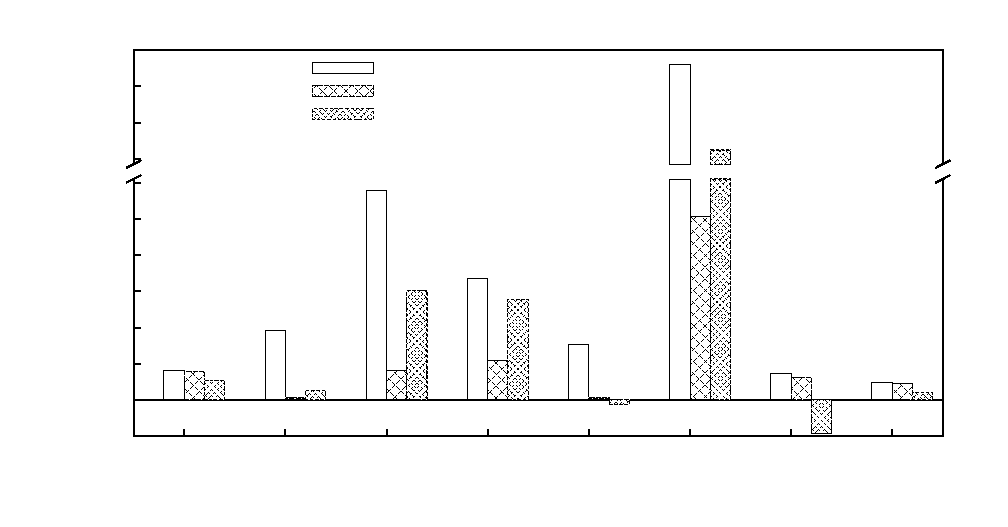
\includegraphics{figures/code_coverage_graph}}%
    \gplfronttext
  \end{picture}%
\endgroup
}
  \caption{Visual representation of the percentage increase of code
    coverage over the baseline scanner, \wget{}. Important to note is
    the gain our scanner, \crawler{}, has over \waf{}, because the
    only difference is our state-aware crawling. The $y$-axis range is
    broken to reduce the distortion of the \wackopicko{} results. }
  \locallabel{code-coverage-graph}
\end{figure}


Table~\localref{code-coverage} shows the results of each of the black-box web
vulnerability scanners against each web application. The column ``\%~over Baseline''
displays the percentage of code coverage improvement of the scanner against the
\wget{} baseline, while the column ``Vulnerabilities'' shows total number of reported
vulnerabilities, true positives, unique true positives among the scanners, and
false positives. 

The prototype implementation of our \crawler{} had the best code coverage for
every application. This verifies the validity of our algorithm: Understanding
state is necessary to better exercise a web application.

Figure~\localref{code-coverage-graph} visually displays the code coverage percent
improvement over \wget{}. The most important thing to take from these results
is the improvement \crawler{} has over \waf{}. Because we use the fuzzing
component of \waf{}, the only difference is in our state-aware crawling. The
results show that this gives \crawler{} an increase in code coverage from as
little as half a percent to 140.71 percent.

Our crawler discovered three unique vulnerabilities (vulnerabilities that no
other scanner found), one each in \phpbbtwo{},
\scarf{}, and \wackopicko{}. The \scarf{} vulnerability is simply a XSS injection
on the comment form. \waf{} logged itself out before fuzzing the comment page.
\skipfish{} filed the vulnerable page under ``Response varies
randomly, skipping checks.'' However, the content of this page does not vary
randomly, it varies because \skipfish{} is altering it. This \emph{random} categorization also prevents
\skipfish{} from detecting the simple XSS vulnerability on \wackopicko{}'s
guestbook. This result shows that a scanner needs to understand the web application's
internal state to properly decide \emph{why} a page's content is changing. 

Skipfish was able to discover 15 vulnerabilities in \vanillaforums{}. This is
impressive, however, 14 stem from a XSS injection via the referer header on an
error page. Thus, even though these 14 vulnerabilities are on different pages,
it is the same root cause. 

Surprisingly, our scanner produced less false positives than \waf{}. All of
\waf{}'s false positives were due to faulty timing detection of SQL injection
and OS commanding. We believe that using HtmlUnit prevented our scanner from
detecting these spurious vulnerabilities, even though we use the same fuzzing
component as \waf{}.

Finally, our approach inferred the state machines of the evaluated
applications. These state machines are very complex in the large applications.
This complexity is because modern, large, application have many actions which modify the
state. For instance, in \wackopicko{}, a user can log in, add items to their
cart, comment on pictures, delete items from their cart, log out of the
application, register as a new user, comment as this new user, upload a
picture, and purchase items. All of these actions interact to form a complex
state machine. The state machine our scanner inferred captures this complex
series of state changes. The inferred \wackopicko{} state machine is presented
in Figure~\localref{wackopicko-state-graph}.

\begin{figure*}[t!b]
  \centering
  \includegraphics{figures/wackopicko.ps}
  \caption{State machine that \crawler{} inferred for \wackopicko{}.}
  \locallabel{wackopicko-state-graph}
\end{figure*}


\section{Limitations}

Although dynamic page generation via JavaScript is supported by our crawler as allowed by the HtmlUnit
framework~\cite{htmlunit}, proper AJAX support is not implemented. This means that our prototype
executes JavaScript when the page loads, but does not execute AJAX calls when
clicking on links.

Nevertheless, our approach could be extended to handle AJAX requests. In fact,
any interaction with the web application always contains a request and
response, however the content of the response is no longer an HTML page. Thus,
we could extend our notion of a ``page'' to typical response content of AJAX
calls, such as JSON or XML. Another way to handle AJAX would be to follow a
Crawljax~\cite{mesbah09:crawljax} approach and covert the dynamic AJAX calls
into static pages.

Another limitation of our approach is that our scanner cannot be used against a
web application being accessed by other users (i.e., a public web application), because
the other users may influence the state of the application (e.g., add a comment
on a guestbook) and confuse our state change detection algorithm. 


\section{Conclusion}

We have described a novel approach to inferring, as much as possible, a web
application's internal state machine. We leveraged the state machine to drive the
state-aware fuzzing of web applications. Using this approach, our crawler is
able to crawl---and thus fuzz---more of the web application than a classical
state-agnostic crawler. We believe our approach to detecting state change by
differences in output for an identical response is valid and should be adopted by
all black-box tools that wish to understand the web application's
internal state machine.

%% \section*{Acknowledgements}
%% This work was supported by the Office of Naval Research (ONR) under Grant
%% N000141210165, the National Science Foundation (NSF) under grant CNS-1116967,
%% and by Secure Business Austria.


% vim:spell:tw=80:sw=1
